\section{Dimensionierung PID Regler nach Kuhn}
Die PID-Reglereinstellung nach Kuhn gibt die folgende Auslegung vor
\[
	\begin{array}{l@{~}c@{~}l@{\qquad}l}
        K_p & = & \frac{2}{K_s}         & ,K_s = K_{g_n} \\
        T_i & = & 0.8 \cdot T_\Sigma    & ,T_\Sigma \xrightarrow{PT_1} \tau_n \\
        T_d & = & 0.194 \cdot T_\Sigma  & ,T_\Sigma \xrightarrow{PT_1} \tau_n \\
	\end{array}
\]
Die allgemeine Übertragungsfunktion zum PID-Regler lautet
\[
	\frac{U(s)}{E(s)}
	= K_p \left(
		1 + \frac{1}{T_i s}
		+ \frac{T_d s}{\left(\frac{T_d}{N}\right)s + 1}
	\right)
	\qquad , N = 10
\]
Mit den Einstellregeln nach Kuhn ergeben sich für die zwei
Übertragungsfunktionen $G_5(s)$ und $G_7(s)$ die folgenden Parameter.

\subsection{PID-Reglereinstellung für $G_5(s)$}
\[
	\begin{array}{l@{~}c@{~}l}
		K_p & = & 0.4116 \si[per-mode = fraction]{\volt\per\cm} \\
		T_i & = & 56 \si{\second} \\
		T_d & = & 13.58 \si{\second} \\
		N & = & 10
	\end{array}
\]

\subsection{PID-Reglereinstellung für $G_7(s)$}
\[
	\begin{array}{l@{~}c@{~}l}
		K_p & = & 0.3448 \si[per-mode = fraction]{\volt\per\cm} \\
		T_i & = & 78.4 \si{\second} \\
		T_d & = & 19.012 \si{\second} \\
		N & = & 10
	\end{array}
\]

\newpage
\subsection{Testergebnisse}

\begin{figure}[h!]
	\centering
	\begin{subfigure}{0.475\textwidth}
		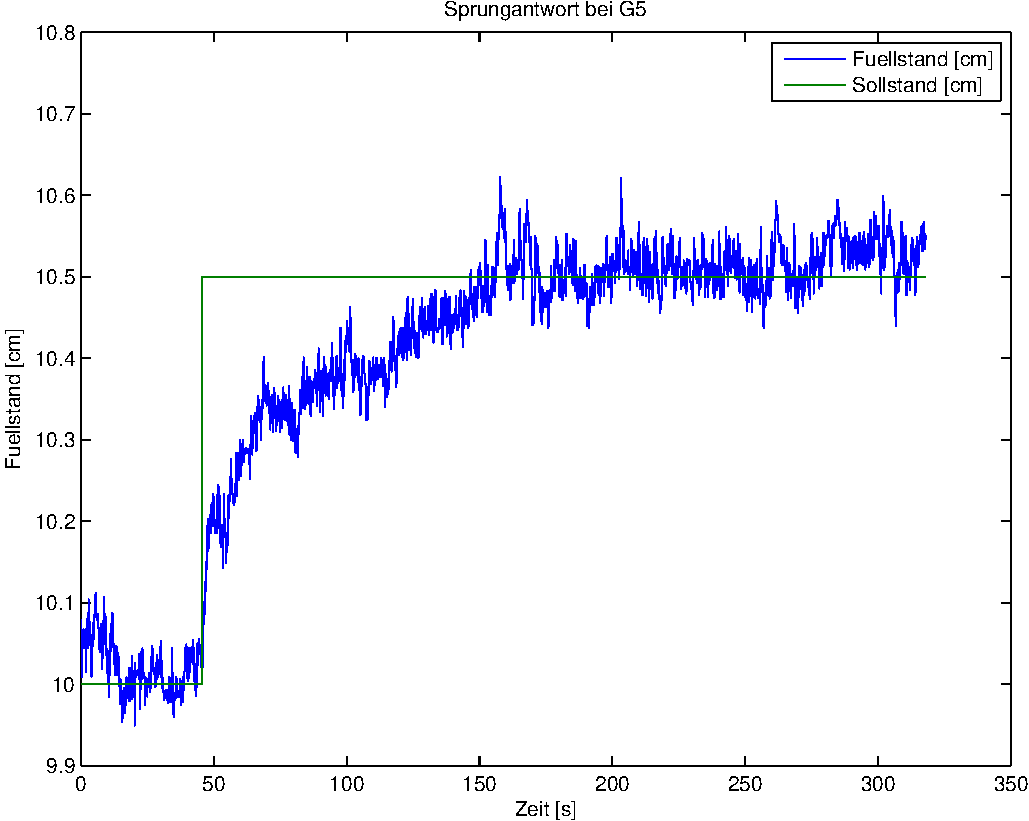
\includegraphics[width=1\textwidth]{09/step_g5_plot.pdf}
		\caption{Sprungantwort bei $G_5(s)$}
	\end{subfigure}
	\hfill{}
	\begin{subfigure}{0.475\textwidth}
		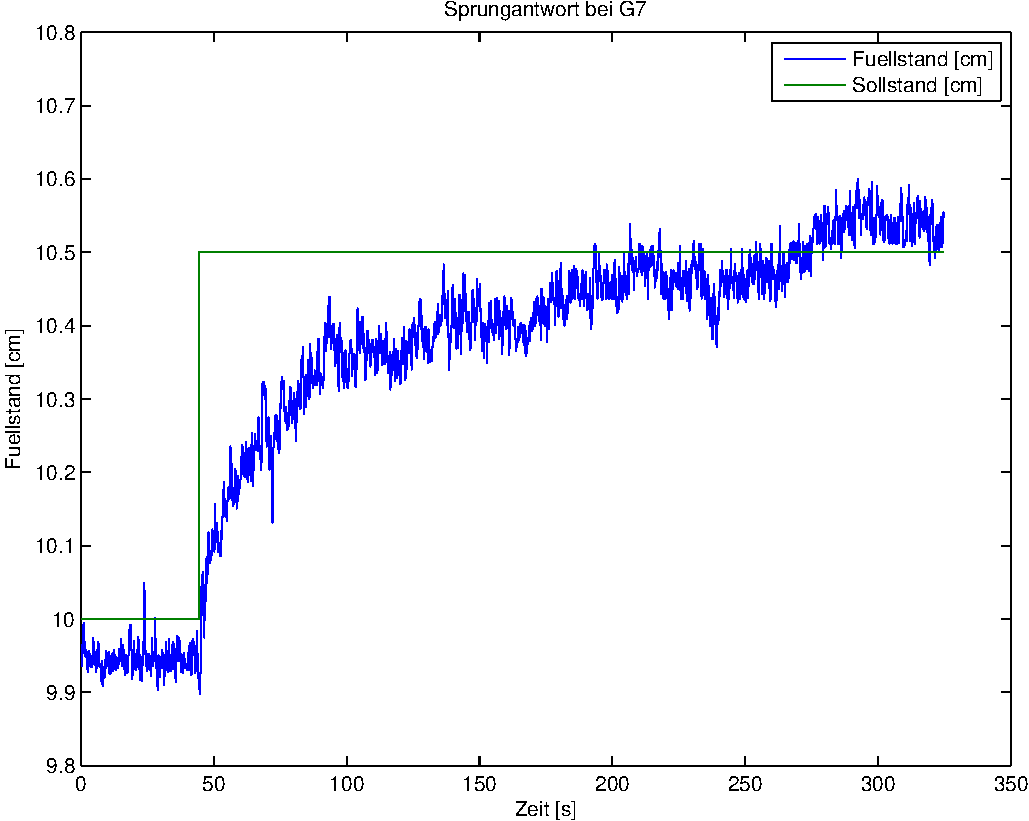
\includegraphics[width=1\textwidth]{09/step_g7_plot.pdf}
		\caption{Sprungantwort bei $G_7(s)$}
	\end{subfigure}
	\caption{Sprungantworten für den PID-Regler nach Kuhn}
\end{figure}

\begin{table}[h!]
	\centering
	\begin{tabular}{l c c c c}
		Eigenschaft
			& Spezifikation
			& bei $G_5(s)$
			& bei $G_7(s)$
			& Einheit \\
		\hline
		Genauigkeit (mean)
			& 100
			& 3.3
			& 8.28
			& \% \\
		Anregelzeit (0-99\%)
			& $4$
			& 106
			& 169
			& $\si{\second}$ \\
		Überschwingen
			& $10$
			& n.a.
			& n.a.
			& \% \\
		Einschwingzeit
			& $5$
			& n.a. 
			& n.a.
			& $\si{\second}$ \\
	\end{tabular}
\end{table}
